%----------------------------------------------------------------------------
\chapter{Mérések}
\label{sec:results}
%----------------------------------------------------------------------------
Ebben a fejezetben szeretném bemutatni a diplomamunka keretein belül elvégzett méréseket és a hozzájuk szükséges egyéb ismereteket.
Először bemutatom milyen lehetőségek voltak a környezet kialakítására és a mérések közben használt eszközöket, szoftverek verzióit.
Ezután következnek a mérések bemutatása és a kapott eredmények értékelése.
Az eredmények kiértékelése során kiderül, hogyan viselkedik forgalomszabályozás nélkül egy szolgáltatásháló és ezen mennyire segít a beépített horizontális skálázó.

%----------------------------------------------------------------------------
\section{Mérés környezete}
%----------------------------------------------------------------------------
A feladat elején főként implementációval kellett foglalkozni így nem kapott jelentős szerepet a Kubernetes klaszter. Ezért  a félév első felében elég volt lokálisan futtatni, amit én Minikube (v1.17.1) segítségével tettem meg. 

Amikor a fejlesztési rész kezdett véglegesedni kellett egy rendes környezet, a rendes mérésekhez. Ehhez több lehetőséget is számításba vettem.	

\begin{itemize}
  \item \textbf{BME Cloud}: Egyik lehetőség az egyetemi felhő volt. Itt létre lehet hozni virtuális gépeket, amiket aztán klaszterbe lehet szervezni. Hátránya viszont, hogy hosszabb távra nehezen lehet gépet igényelni, rendszeresen le is állítják ami könnyen okozhatja egy-egy mérés elvesztését, hiszen több órán keresztül is futhat.
  \item \textbf{Klaszter a felhőben}: Kézenfekvő megoldás lehet igényelni egy teljes, egész klasztert. Erre több opció is van, csak hogy a legnagyobbakat említsem: Google, Amazon, Microsoft. Ezek a minőségi szolgáltatások azonban havidíjasok lennének, és bizonyos tekintetben kevésbé rugalmasak. %TODO: készültek becslések a havidíjra.
    \item \textbf{Tanszéki infrastruktúra}: A tanszéken létezik egy előretelepített klaszter, amin lehetne méréseket készíteni, de általában foglalt.
      \item \textbf{VM igénylés a Schönherz kollégiumtól}: A Villamosmérnöki és Informatikai Karhoz tartozó Schönherz kollégiumban lévő Kollégiumi Számítástechnikai Körtől lehet tanulmányokhoz és egyéb projekthez kapcsolódóan virtuális gépeket igényelni. Az igénylés leadása után lehetőséget kaptam három virtuális gép használatára egészen a projektfeladat végéig. Bizonyos hátulütőkkel ezen lehetőségnél is számításba kellett venni. Ilyen például, hogy öntevékeny körként hiba esetén a többinél lassabb válaszidőkre lehet számítani.
\end{itemize}		

A fenti opciók közül számomra a negyedik volt a legszimpatikusabb így kaptam is három teljesen új virtuális gépet. Telepítéshez a Debian (v10 - Buster) operációs rendszert választottam, mert stabil, megbízható és széles körben támogatott. A virtuális gépek tulajdonságai az \ref{tab:nodes} ábrán láthatóak. Hasonló erőforrásértékekkel rendelkeznek, annyi különbséggel, hogy csak az egyik gépnek van publikus címe. Továbbá a táblázat tartalmazza az egyes csomópontok nevét és a klaszteren belüli szerepét is.

\begin{table}[ht]
\centering
  \begin{tabular}{c|cccc}
	  Tulajdonság & VM 1 & VM 2 & VM 3 \\
    \hline
	CPU (mag) & 4 & 4 & 4 \\ 
	Memória (GB) & 4 & 4 & 4 \\
	Tárhely (GB) & 10 & 10 & 10 \\  
	Node neve & dipterv1 & dipterv2 & dipterv3 \\ 
	Külső IP & 152.66.211.2 & $\varnothing$ & $\varnothing$ \\ 
	Belső IP & 10.151.103.1 & 10.151.103.2 & 10.151.103.3 \\
	K8s szerep& control-plane,master & worker & worker \\
  \end{tabular}
  
  \caption{Használt csomópontok tulajdonságai}
\label{tab:nodes}
\end{table}

\subsection{Klaszter előkészítése}
%----------------------------------------------------------------------------
A virtuális gépekből klasztert kellett szervezni, amire különböző megoldások léteznek.\citep{kubernetesInstall} Két különbözőt szeretnék kiemelni:
\begin{enumerate}
  \item \textbf{Kubespray}: \textit{Ansible} felhasználásával előre definiált lépéseket hajt végre. Mindössze egy pár soros konfigurációt kell írni hozzá és ígérete szerint minden mást elintéz.
  \item \textbf{Kubeadm}: Az előzőhöz képest a \textit{kubeadm} jóval manuálisabb módszer. Segítségével le tudunk generálni mindenféle kulcsot a klaszterhez, csomópontokat bekötni a rendszerbe.
\end{enumerate}

Nem szándékosan de kipróbáltam mindkét megoldást. Vonzó volt ugyanis a Kubespray, hogy könnyen és automatikusan telepít minden függőséget. Sajnos pont amiatt mert ilyen magas szinten vezeti a telepítést hiba esetén nem sok információ derült ki. Miután eredménytelenül zárult minden próbálkozás, újratelepítettem a virtuális gépeket és áttértem a Kubeadm használatára. 

A telepítés menetét nem részletezném, mert a hivatalos weboldalon látható lépéseken kellett végigmenni. Az elkészült klaszter egy mester csomópontot és kettő kiszolgáló csomóponttal rendelkezik. A fő csomópont rendelkezik egyedül külső hálózatról elérhető, publikus IP címmel, a többinek csak belső címen érhetőek el. Ez némiképpen nehezítette a telepítés folyamatát, részben emiatt sem működött a Kubespray megoldása. 

A klaszter elkészülte után még pár függőséget ki kellett elégíteni, hogy a lokálisan összeállított mérő keretrendszer működni tudjon. Külön telepíteni kellett egy konténer hálózati interfészt (CNI). Ez alapból nem jön a Kubernetessel így külön kell installálni, hogy a különböző csomóponton futtatott konténerek tudjanak egymással kommunikálni. A választás a \textit{Cilium} szoftverre esett, mert szerettem volna jobban megismerni, széleskörűen használható és jól dokumentált. Telepítése után lehetőségünk van teszteseteket futtatni, ami igazolja a klaszterben a csomópontok és kapszulák kommunikációját. 

A \ref{sec:measure_orchestrate} szakaszban leírt módon a mérések során gyűjtött adatok jelentős részét a Prometheus rendszere gyűjti össze és tőle kérdezzük le. Emiatt az éles méréseket végző klaszterben is telepíteni kellett. Ebben a Helm, Kuberneteshez készített csomagkezelő megoldása segített. A \verb+prometheus-stack+ csomagot kellett telepíteni annyi kiegészítéssel, hogy kintről is elérhetővé tegyük a felületet és szolgáltatásait. Azt úgy érhetjük el, hogy a létrehozandó \verb+Service+  típusát \verb+NodePort+-ra állítjuk és a következetesség miatt adunk neki egy portszámot. Az így létrehozott környezet rendelkezik egy webes felhasználói felülettel is, ahol tetszőleges lekérdezéseket indíthatunk. Egy ilyen lekérdezés látszik az \ref{fig:prometheus_example} ábrán is. A példán az látszik, hogy milyen eredményt kapunk, ha lekérdezzük az aktuálisan futó kapszulákat a \verb+Default+ és \verb+Metrics+ névtérben. Az eredményből leolvasható, hogy jelenleg 3 darab \textit{back-end}, 2 darab \textit{front-end} és 1 darab \textit{db} névvel ellátott konténer fut. \\

% Prometheus példa -------------------------------------------------------
\begin{figure}[!ht]
\centering
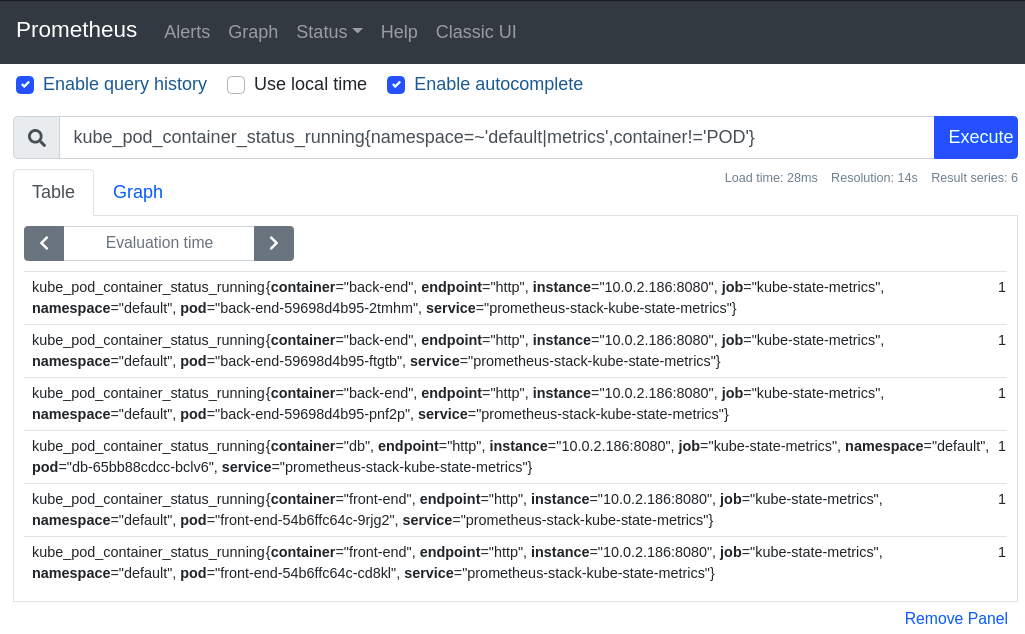
\includegraphics[width=150mm, keepaspectratio]{figures/prometheus_example.png}
\caption{Telepített \textit{Prometheus} rendszere}
\label{fig:prometheus_example}
\end{figure}

Az aktuális rendszerben az operátor még nem külön konténerként fut egy kapszulában, hanem a klaszteren kívül, lokálisan a szerveren, mint egy Go alkalmazás. Emiatt külön telepíteni kellett a Go nyelvet is, hogy el tudjon indulni a rendszer.

\subsection{Verziók}
%----------------------------------------------------------------------------
A rendszer és mérések összeállításához több különböző komponenst kellett integrálni.
Az \ref{tab:versions} táblázat összefoglalóan tartalmazza az egyes környezetek és használt eszközök verzióit. 
Mindig törekedtem a legfrissebb verzió használatára, hiszen ezek tartalmazzák a legtöbb funkciót és a legtöbb hibajavítást, azonban a környezet összeállítása után már végeztem verziófrissítést, nehogy eltérést okozzon a mérési eredményekben.

\begin{table}[ht]
\centering
  \begin{tabular}{l l}
	  Szoftver 		& Verzió \\
    \hline
      Go 			& 1.16.3 \\ 
      Kubernetes 	& 1.21.0 \\ 
      Kubectl 		& 1.21.0 \\
      Cilium 		& 1.9.5 \\
      Python 		& 3.7.3 \\ 
      Prometheus 	& 2.24.0 \\ 
      Grafana 		& 7.5.3 \\ 
      Operator-SDK 	& 1.4.0-32 \\ 
      Debian 		& 10 (buster)  \\ 
      Istio			& 1.11.4 \\
  \end{tabular}
  
  \caption{Használt verziók}
\label{tab:versions}
\end{table}


%----------------------------------------------------------------------------
\section{Példa mérés}
%----------------------------------------------------------------------------
A rendszer összeállítása után lehetővé vált konkrét mérések elvégzése.
A rendszer működését bizonyítandó és az egyes elemek további finomhangolása miatt kezdetben egy példa mérésen kísérleteztem.
A mérésnek nem volt célja a hasznos eredmények gyűjtése, csak az elvárt működés bizonyítása. 
Főleg ezen mérés alatt derült ki, hogy a korábban használt forgalomgenerátor alkalmazást is le kell cserélni, ezzel is közelebb kerülve a valósághű eredményekhez.

A szimulációban két szolgáltatás vett részt, melyek \aref{fig:sample_sg} sorszámú ábrán is láthatóak.
Volt egy nodeport segítségével kintről elérhető \textit{front-end} szolgáltatás, illetve egy csak bentről elérhető \textit{back-end}.
Azt a szituációt vizsgáltuk, amikor a \textit{front-end} nem használ sok erőforrást, és két pod fut belőle.
Ezzel szemben a \textit{back-end} egy jóval erőforrás igényesebb szolgáltatás, viszont három egység fut belőle.
A \textit{front-end} minden felé érkező, \verb+/to-backend+ végpontra érkező kérést továbbított a \textit{back-end} \verb+heavy+ végpontjára.
A hálózattal elértük, hogy a második szolgáltatásunk a számára beállított, sok processzort igénylő műveletet hajtsa végre.

% Példa szolgáltatás háló----------------------------------------------------
\begin{figure}[!ht]
\centering
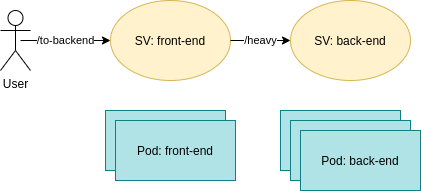
\includegraphics[width=100mm, keepaspectratio]{figures/sample_measurement.png}
\caption{A mérésnek kitett szolgáltatások kapcsolata}
\label{fig:sample_sg}
\end{figure}

A kapott eredményekből készült grafikon látható az \ref{fig:example_plot} és \ref{fig:example_responsetime} ábrákon. 

A kapott \ref{fig:example_responsetime} ábráról leolvasható, hogy az átlagos válaszidő a mérés során nem változott érdemben, végig kellően alacsony maradt.
Fontos megjegyezni, hogy a mérés során nem vittünk a rendszerbe mesterséges késleltetést, csak a kötelező műveletek elvégzését vártuk meg, így jött ki az állandó válaszidő.

A másik, \ref{fig:example_plot} grafikonon látható, hogy a kevésbé erőforrás-igényes \textit{front-end} processzor felhasználása lassan de folyamatosan nő egészen addig, amíg a \textit{back-end} is tudja növelni a processzor felhasználását. Ez körülbelül 125 QPS-ig tart. Ilyenkor a \textit{back-end} eléri az indításkor beállított erőforrás limitációt és emiatt nem tud több beérkező igényt kiszolgálni.  Emiatt a felhasználói forgalmat generáló alkalmazás sem fog tudni több kérést a rendszer felé küldeni, mert meg kell várja, mire a \textit{front-end} válaszol, de a front-end csak azután válaszol, hogy meghívta a végletekig megterhelt \textit{back-end} szolgáltatást.
A szimulációhoz még a korábbi verziókban használt \textit{Fortio} generálta a klaszter számára a forgalmat, azonban a működése nem egyezett a valóságban feltételezhető viselkedéssel.
Valóságban a klaszter terheltségétől függetlenül fognak az új kérések érkezni és nem a sikeresen kiszolgált kérések számától.
Ez is egy kiváltó oka volt a \textit{Vegetára} történő váltásnak.

Érdemes figyelembe venni, hogy az $X$ tengely az igényelt lekérdezések darabszámát mutatja, nem a rendszer által valóságban kiszolgált kérések mennyiségét.
 \\


% Generált példa ábrák -------------------------------------------------------
\begin{figure}[!ht]
\centering
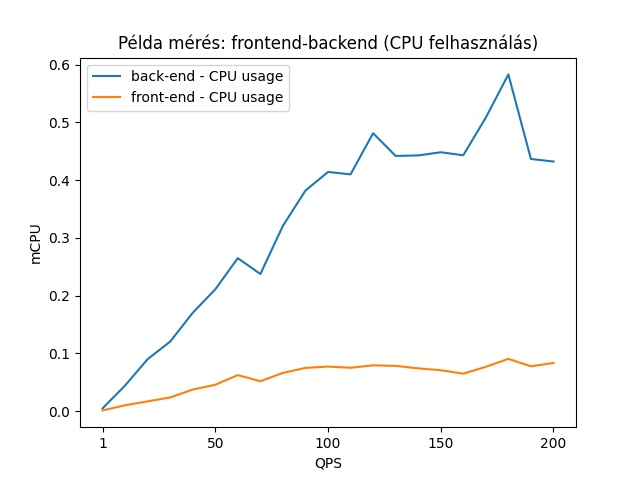
\includegraphics[width=150mm, keepaspectratio]{figures/sample_plot_cpu.jpg}
\caption{\textit{Front-end} és \textit{back-end} egységből álló rendszer CPU felhasználása}
\label{fig:example_plot}
\end{figure}

\begin{figure}[!ht]
\centering
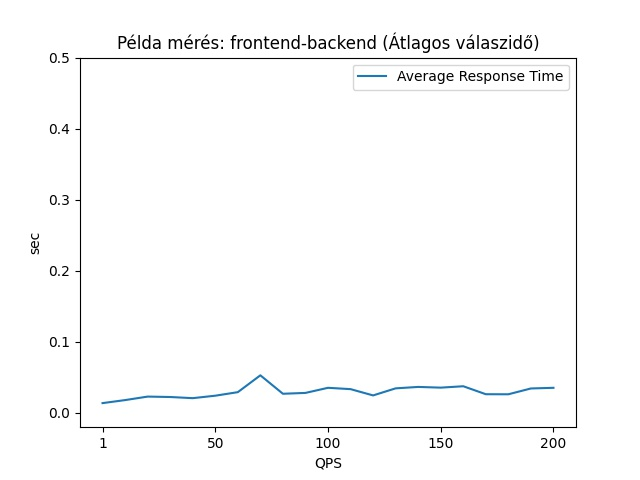
\includegraphics[width=150mm, keepaspectratio]{figures/sample_plot_responsetime.jpg}
\caption{\textit{Front-end} és \textit{back-end} egységből álló rendszer átlagos válaszideje}
\label{fig:example_responsetime}
\end{figure}

%----------------------------------------------------------------------------
\section{Tervezett mérések}
%----------------------------------------------------------------------------
A korábban bemutatott mérés alapján a rendszer képes szimulációkat futtatni és a kapott adatokat feldolgozni.
Ezután meg kellett tervezni a diplomamunkához szükséges méréseket, amik a lehető legtöbb információval fognak szolgálni.

\begin{itemize}
	\item \textbf{Szolgáltatásháló HPA nélkül} - Szükséges méréseket végezni, hogy megértsük a szolgáltatáshálók alapvető kiszolgálási működését. Az itt elvégzett méréseket lehet később referenciának használni.
	\begin{itemize}
		\item[$\circ$] \textbf{3 frontend egymás után, 1 backend} - A beérkező kérés kiszolgálása  egy szolgáltatásokból álló láncon halad végig. A lánc eleje tartalmazza a gyors, nem erőforrás műveleteket és a lánc végén kerül sor a költséges műveletre. 
		
		\item[$\circ$] \textbf{3 frontend egymás mellett, 1 backend} - Az előzővel hasonló architektúra, azonban a frontend szolgáltatást megvalósító alkalmazások egymás mellett helyezkednek el, így a láncolat hossza lecsökken és az általuk kiszolgált kérések száma növekedhet.
	\end{itemize}
	
	\item \textbf{Szolgáltatásháló HPA segítségével} - A referencia mérések után meg kell nézni, milyen változásokat érhetünk el a beépített automatikus skálázóval.
	
	\begin{itemize}
		\item[$\circ$] \textbf{1 frontend, 1 backend egymás után} - A mérés során megfigyeljük, hogy a kezdeti konfigurációval hogyan változnak a kezelt alkalmazáskomponensek száma. Ki fog derülni, maximálisan mennyi pod futhat egyszerre. 
		
		\item[$\circ$] \textbf{Korábbi mérés több konfiguráció mellett} - Az előző pontban kapott eredmények alapján a szükséges konfigurációk módosítása mellett figyeljük a szimuláció során kinyert eredményeket. Módosítjuk a kezdeti replikaszámot és a cél processzorhasználati értéket is.
		
	\end{itemize}
	
\end{itemize}


%----------------------------------------------------------------------------
\section{Elvégzett mérések statikus konfigurációkkal}
%----------------------------------------------------------------------------
A projektmunka jelentős részét tette ki, hogy méréseket kellett végezni a korábban bemutatott rendszerelemekkel rendelkező környezetben.
A mérések darabszámát szemlélteti \aref{number_of_measurements} kódrészlet. Beépített Linux parancsok segítségével könnyen megkaphatjuk a projekt során készített és a kiértékeléshez használt \textit{json} dokumentumok darabszáma. Ahogy a kódrészlet is mutatja először rekurzívan lekérdezzük az adott mappán és almappákon belül található adott kiterjesztéssel rendelkező fájlokat \textit{(find)}. 
Majd az így kapott eredményt csővezeték segítségével hozzákötjük egy szintén beépített parancs \textit{(wc)} bemenetére, ami megszámolja a kiírt sorok számát. 
Ahogy az a kódrészleten is látszik, hogy ennek a kimenete $1445$, ami azt jelenti, hogy a projekt jelenlegi állapotához kapcsolódóan ennyi mérés született. %TODO konkrét mérési számot frissíteni
Az egyes mérések itt egy-egy Vegeta terheléshez kapcsolódó konfigurációk, válaszidők és egyéb Prometheus-ból kapott eredményeket jelenti.

% Mérések számának meghatározása --------------------------------------------
\lstset{caption=Elvégzett mérések száma, label=number_of_measurements}
\lstinputlisting{figures/get_number_of_measuremnts.sh}

A következő alfejezetekben szeretném bemutatni azon méréseket, amelyek nem tartalmaztak semmilyen automatikus mechanizmust, ezáltal a nem tudták a terheléstől függően módosítani a konfigurációikat.
A fő kérdés az volt, hogyan viselkedik a rendszer külső forgalomszabályozás (\textit{flow control}) nélkül.
Alapértelmezetten nincsen limitáció a klaszterbe érkező kérések számára illetve az egyes szolgáltatásokhoz érkező kérésekre sem, ezért lehetőségünk van elárasztani azokat.
A szimulációk során folyamatosan növelve a beküldött kéréseket figyeljük a rendszer kiszolgálási paramétereit és stabilitását.

\subsection{Költséghatékony frontendek és költséges backend láncban}
\label{subsec:3FE_1BE_chain}
%----------------------------------------------------------------------------
Az első bemutatott mérésnél azt vizsgáltam, hogyan változik a rendszer működése, ha több költséghatékony alkalmazáson keresztül jut el egy erőforrás-igényes hátsó alkalmazáshoz.
A szimulált szolgáltatáshálót alkotó elemek \aref{tab:3FE_1BE_chain} táblázatban bemutatott specifikációkkal rendelkeznek.
Látható, hogy a három költséghatékony frontend egymásnak továbbítják a beérkező kéréseket, majd ezután jut el a backendhez.
A könnyebb értelmezés miatt mindegyikből egy darab replika került elindításra. 
A frontend egységek egy-egy kérés kiszolgálásához nagyjából 10mCPU processzort igényelnek, és 1000mCPU volt a lefoglalt és a maximálisan felhasználható erőforrás mennyiség számukra.
Ezek alapján $\frac{1000 mCPU}{10 mCPU/kérés} = 100 kérés$ kiszolgálására elegendő erőforrás van számukra allokálva.
Ezzel szemben, a sor végén álló, költséges backend maximum 2vCPU-t használhat, és az egyes beérkező lekérdezések kiszolgálására 100 mCPU processzorra van szüksége.
Ebből kifolyólag maximum $\frac{2000 mCPU}{20 mCPU/kérés} = 20 kérés$ kiszolgálására van lehetőség másodpercenként. 

Minden kérés a \textit{front-end-1}-hez érkezik be és innen kerül továbbításra. 
Mivel a sor elején lévő egységek ötször több kérést tudnak kiszolgálni, ezért a szűk keresztmetszet a sor hátulján lévő \textit{back-end-1} lesz.
Emiatt minden beérkező kérésnek el kell jutnia a sor végére, miközben a sor elején lévő egységeken erőforrás-használatot indukál.
Mire eljut a sor végére és feldolgozásra kerül, addig a beérkező \textit{http} kapcsolat eldobásra is kerülhet a beállított öt másodperces időkorlát miatt.

\begin{table}[ht]
\centering
\begin{tabular}{l|llll}
Név                                                            & front-end-1    & front-end-2    & front-end-3   & back-end-1 \\ \hline
Replikák száma                                                 & 1              & 1              & 1             & 1          \\
\begin{tabular}[c]{@{}l@{}}CPU használat\\ (mCPU)\end{tabular} & 10             & 10             & 10            & 100        \\
\begin{tabular}[c]{@{}l@{}}CPU limit\\ (mCPU)\end{tabular}     & 1000           & 1000           & 1000          & 2000       \\
\begin{tabular}[c]{@{}l@{}}Memória limit\\ (kB)\end{tabular}   & 1000           & 1000           & 1000          & 1000       \\
Továbbhívás                                                    & front-end-2:80 & front-end-3:80 & back-end-1:80 & -         
\end{tabular}
  	\caption{Három költséghatékony frontend után egy költséges backend}
	\label{tab:3FE_1BE_chain}
\end{table}

Az ismertetett környezetben elvégzett mérésről készített grafikon látható \aref{fig:3FE_1BE_chain} ábrán.
Megfigyelhető, hogy az egyre nagyobb beérkezett terhelés hatására folyamatosan növekszik a rendszer által felhasznált erőforrások mennyisége.
Különösen érdekes, hogy a \textit{back-end-1} által használt processzor mennyisége, a várt módon, 20 lekérdezés / másodperc érték környékén eléri a maximumot, onnan már nem emelkedik tovább, csak stagnál. 
Ezzel ellentétben az egyes frontend alkalmazások erőforrásigénye folyamatosan növekszik a mérés végéig.

Ezzel párhuzamosan a memória használata is érdekesen alakul.
18 QPS értékig látszólag nem változik érdemben, alacsonyan marad.
Azonban a backend telítése után, minden egységnél elkezd növekedni.
Ez azzal magyarázható, hogy a rendszerben lévő várakozási sorok, pufferek folyamatosan telnek meg, mivel a láncolat végén lévő költséges backend nem képes a beérkezések számával tartani a kiszolgálási számot. 
%TODO - Markow láncok / tömegkiszolgálással magyarázni.  http://www.szit.bme.hu/~gyorfi/tomkisz.pdf

Az alsó sorban látható grafikonok segítségével leolvasható, hogy az átlagos válaszidők 20 QPS környékén elérik az 5 másodperces felső korlátot, amivel szinkronban az időben kiszolgálásra kerülő kérések száma is drasztikusan elkezd visszaesni, majd utána a beérkező kérések elhanyagolható részét tudjuk csak időn belül kiszolgálni. 
Összességében megállapítható, hogy létezik egy olyan pont a szimulációban, aminél több beérkező kérés esetén csak az erőforrásokat használjuk és az érdemi kiszolgálás is hirtelen és drasztikus mértékben visszaesik.
Ilyenkor elszállnak a késleltetések és memória használat, valamint folyamatosan nő a processzor használata is.

\begin{figure}[!ht]
	\centering
	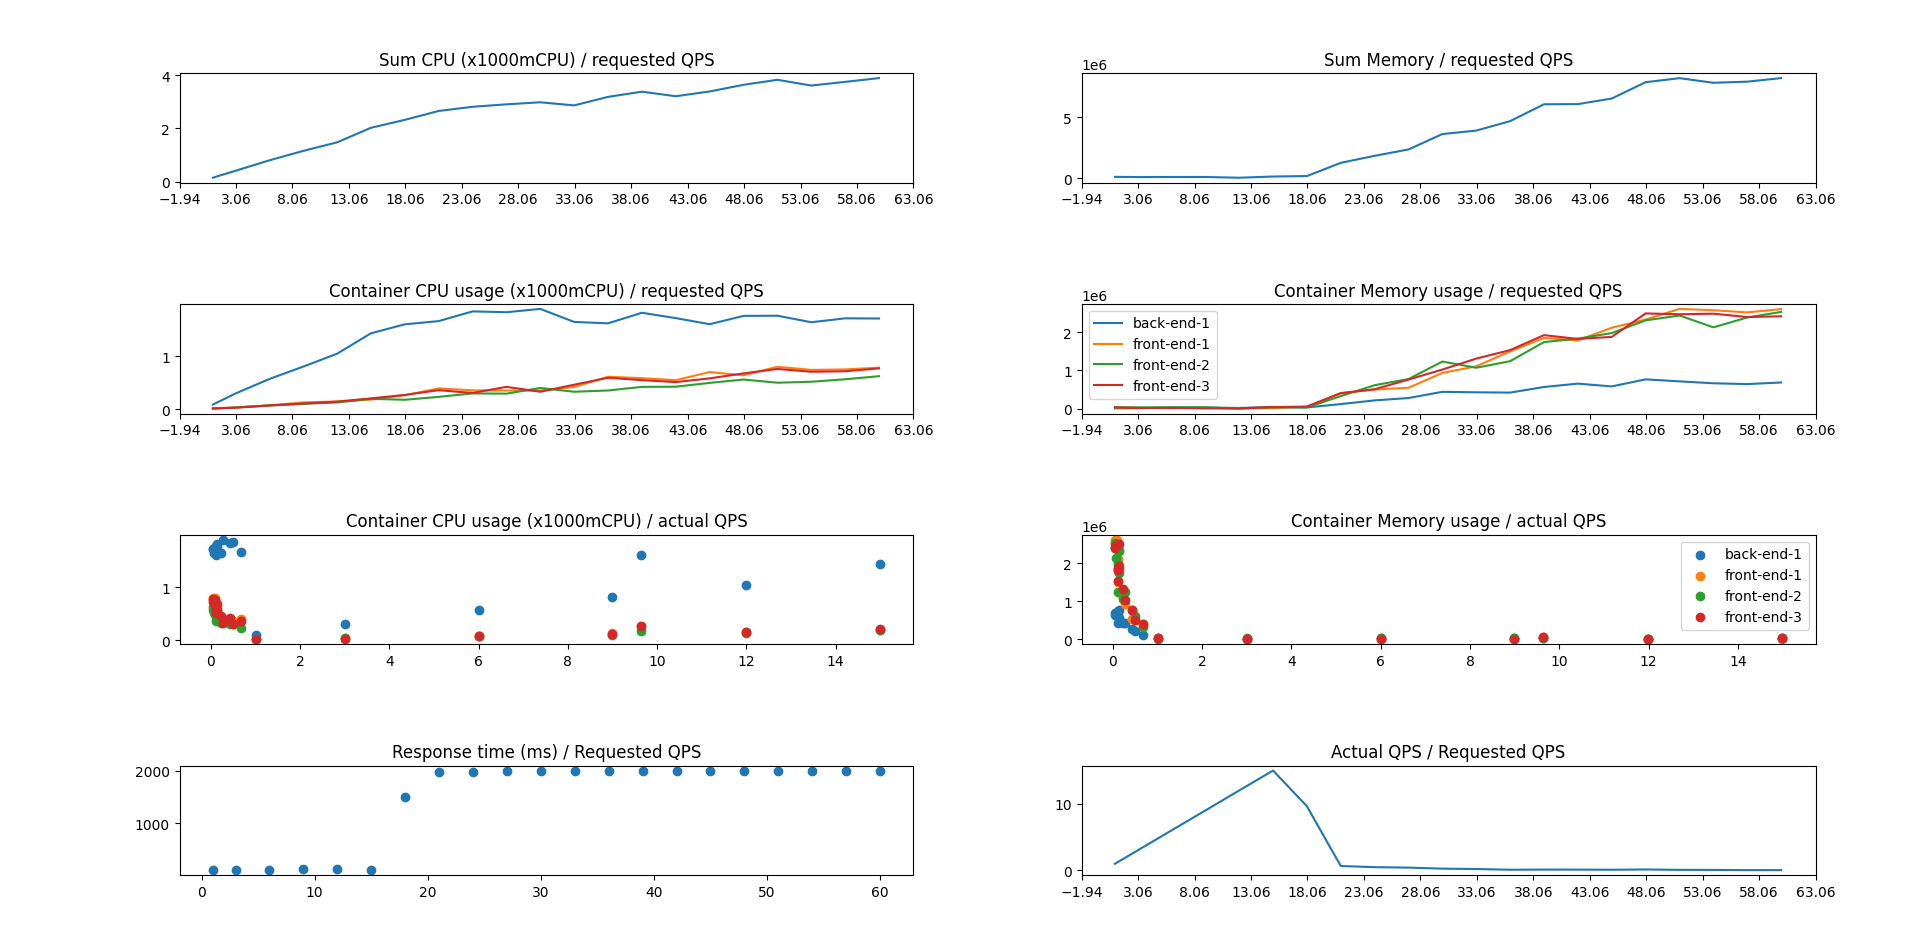
\includegraphics[width=150mm, keepaspectratio]{figures/taildrop-chain-3FE-1BE_requestedQPS.png}
	\caption{Három költséghatékony frontend után egy költséges backend mérés ábrázolása}
	\label{fig:3FE_1BE_chain}
\end{figure}

\subsection{Költséghatékony frontendek egymás mellett és költséges backend mögöttük}
\label{subsec:3FE_1BE_stack}
%----------------------------------------------------------------------------
\Aref{subsec:3FE_1BE_chain} fejezetben látott eredmények alapján felmerült a kérdés, hogyan változnak a kiszolgálási paraméterek, a rövidebb szolgáltatásháló esetén. 
Emiatt a hálózat architektúráját módosítani kellett.
A megkonstruált erőforrás-használatok és a rendszer felépítését \aref{tab:3FE_1BE_new} táblázat tartalmazza. 

Látható különbség, hogy ebben a mérésben nem hozunk létre egy hosszú láncot az egyes frontend alkalmazások egymás mögé kötésével, hanem ennél sokkal rövidebb lesz egy-egy kérés kiszolgálásának folyamata. 
A költséghatékony frontend után rögtön a költséges backendhez kerül továbbításra a beérkező kérés.
Ezen kívül még egy fontos módosítás, hogy három darab frontend fog futni és továbbra is egy backend lesz hátul.
A megadott alapján kiszámolható az egyes egységek által körülbelül kiszolgálható kérések száma másodpercenként.
\refstruc{eq:3FEsumqps} alapján leolvasható, hogy a \textit{front-end-1} áteresztő képessége 120 kérés, míg a \textit{back-end-1} ennél jóval szerényebb 20 beérkező kérést tud kiszolgálni másodpercenként, mint ahogy az következik \aref{eq:1BEsumqps} egyenletből.

\begin{equation}
\label{eq:3FEsumqps}
3(replika)\times\frac{1000 mCPU}{25 mCPU/kérés} = 120 kérés/másodperc
\end{equation}

\begin{equation}
\label{eq:1BEsumqps}
1(replika)\times\frac{2000 mCPU}{100 mCPU/kérés} = 20 kérés/másodperc
\end{equation}

\begin{table}[]
\centering
\begin{tabular}{l|ll}
Név                                                            & front-end-1   & back-end-1 \\ \hline
Replikák száma                                                 & 3             & 1          \\
\begin{tabular}[c]{@{}l@{}}CPU használat\\ (mCPU)\end{tabular} & 25            & 100        \\
\begin{tabular}[c]{@{}l@{}}CPU limit\\ (mCPU)\end{tabular}     & 1000          & 2000       \\
\begin{tabular}[c]{@{}l@{}}Memória limit\\ (kB)\end{tabular}   & 1000          & 1000       \\
Továbbhívás                                                    & back-end-1:80 & -          \\
HPA                                                            & -             & -         
\end{tabular}
  	\caption{Költséghatékony frontend több replikával és utána egy költséges backend}
	\label{tab:3FE_1BE_new}
\end{table}

Jelen mérésben nincsen megadva semmilyen automatikus skálázó, ezért amikor az operátor az indításkor létrehozza adott replikaszámmal az egyes Kubernetes Deploymenteket, azok nem is fognak változni, függetlenül a beérkező kérések mennyiségétől.
A korábban bemutatott környezeten is elvégeztem a szimulált terheléssel történő mérést.
Ezen eredményeket mutatja be \aref{fig:3FE_stack_1BE} ábra.
A korábbi méréssel szinkronban, hasonló megállapításokat tudunk leolvasni.
Látható, hogy a \textit{back-end-1} telítése az elvárt 20 QPS körül megtörténik (illetve kicsit még előtte). 
Azonban ettől függetlenül a \textit{front-end-1} által elhasznált processzor mennyisége folyamatosan nőtt. A legmagasabb terhelésnél már olyan szintre emelkedett a három példány által összesen használt processzor erőforrása, mint a backend maximuma, tehát mintha 2 teljes virtuális CPU magot is lefoglaltunk volna számukra.

A költséges backend telítése után jelentősen megugrik a beérkező kérések kiszolgálásához szükséges késleltetések és az egyes egységek által használt memória mennyiségek is.
A jobb alsó grafikonon látszik, hogy 20 QPS-nél már vissza is zuhant a sikeres kiszolgálások száma, amivel szinkronban a kiszolgálások átlagos válaszideje is megugrik a maximumra, ami jelenleg 5 másodperc, mert a beállítások szerint ennyi idő után bontjuk a \textit{http} kapcsolatokat.

\begin{figure}[!ht]
	\centering
	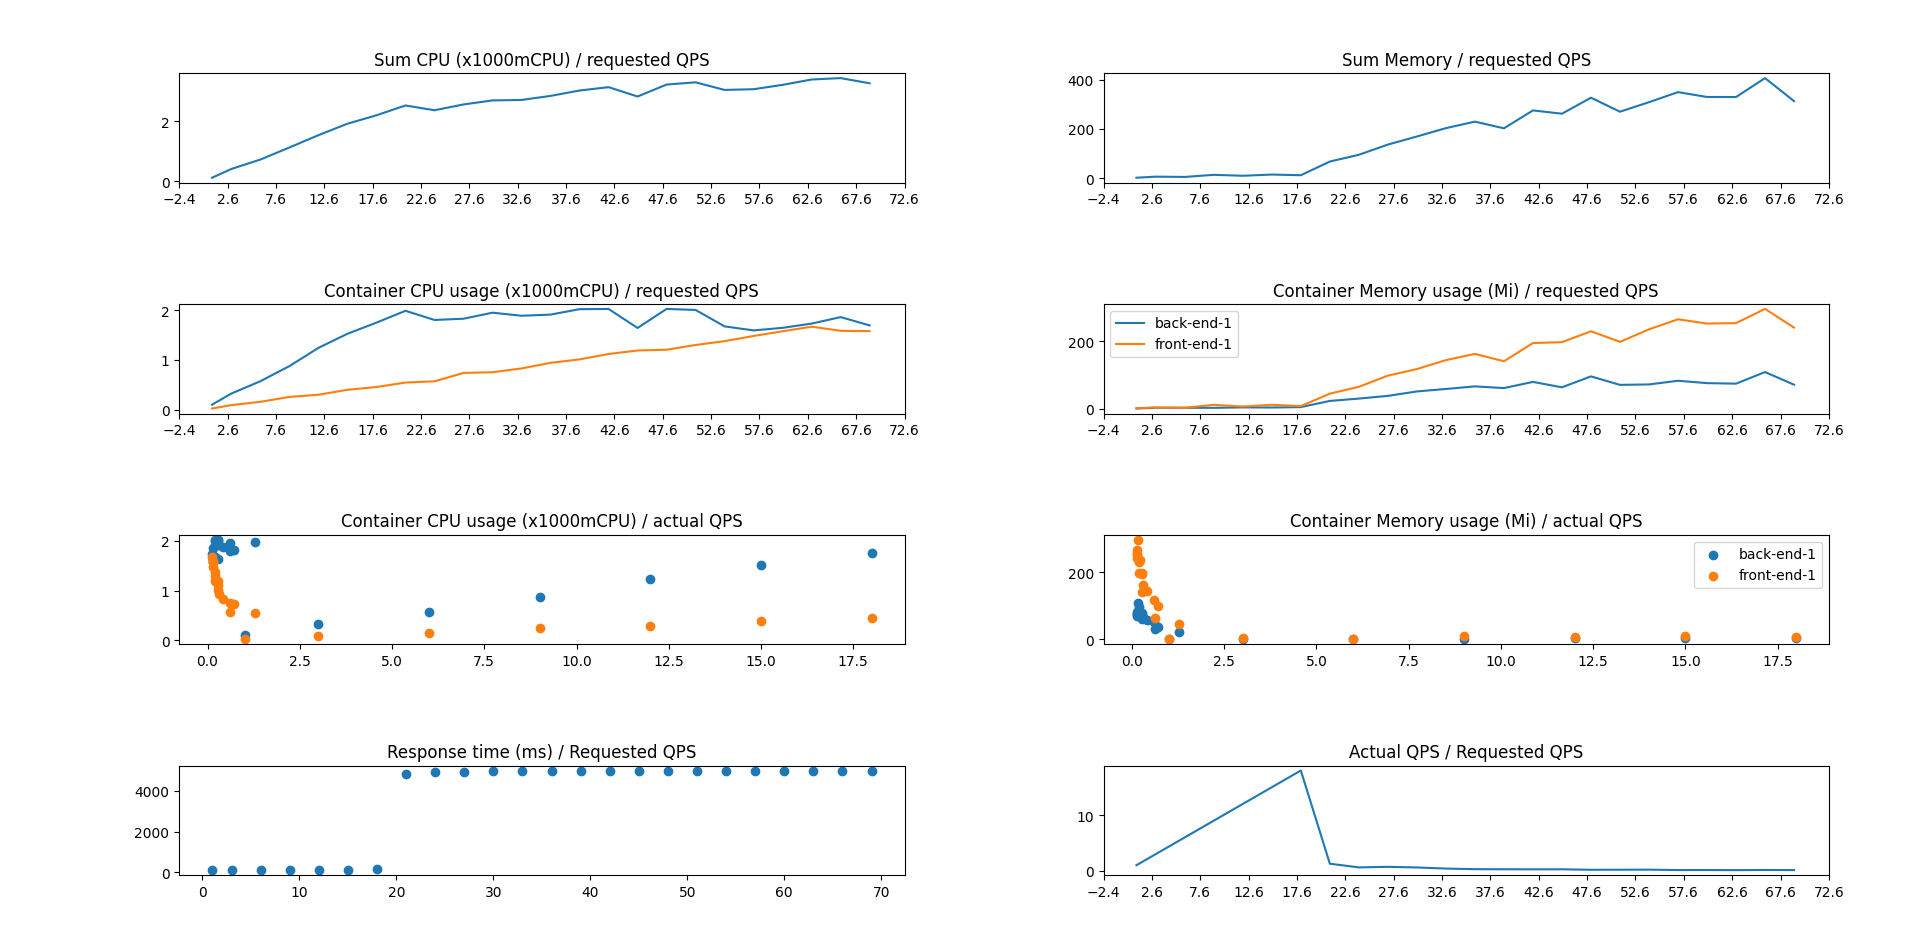
\includegraphics[width=150mm, keepaspectratio]{figures/multiFE-singleBE.png}
	\caption{Költséghatékony frontend három példányban és utána egy költséges backend mérés ábrázolása}
	\label{fig:3FE_stack_1BE}
\end{figure}

Röviden elmondható, hogy a beérkező kérések növelésével együtt fokozatosan nő az elhasznált processzor mennyisége és a sikeres kiszolgálások száma is.
Azonban van egy pont, amikor a hálózatban lévő szűk keresztmetszet nem képes tartani a lépést a beérkező kérések mennyiségével. 
Ebben az esetben hirtelen visszaesik a kiszolgálás minősége, drasztikusan megugrik a várható kiszolgálási idő és ezzel együtt csökken a sikeres kiszolgálások aránya.


\subsection{Tapasztalt probléma összegzése}
%----------------------------------------------------------------------------
Az elvégzett mérések válaszul szolgáltak a kérdésre, hogy mi történik statikus konfiguráció esetén a szolgáltatásháló kiszolgálási teljesítményeivel, ha nagy mennyiségű kiszolgálandó kérés érkezik be.
Látható, hogy forgalomszabályozás nélkül túlterhelődik a hálózatban szereplő szűk keresztmetszet, ami ezután drasztikusan kihat a teljes rendszer működésére.
Mivel nincsen mechanizmus ennek az észlelésére, ezért nagyobb terhelés esetén a korábbi mennyiségű kérés kiszolgálása sem lesz lehetséges, ez okozza a sikeres kiszolgálások csökkenését.

A probléma orvoslására több megoldási irány is létezik. 
Ilyen például a rendelkezésre álló erőforrások optimálisabb elosztása, a túlterhelt egység skálázása vagy a hálózati forgalom szabályozása.
Ha a beállítások dinamikusabbak lennének, akkor a frontend által lefoglalt és feleslegesen használt erőforrásokat át lehet csoportosítani a backend részére, amivel növelhető lenne a rendszer globális maximum kiszolgálása.

Belátható, hogy egy valóságban előforduló problémáról van szó, amelynek vizsgálata indokolt.

%----------------------------------------------------------------------------
\section{Mérések automatikus horizontális skálázóval}
%----------------------------------------------------------------------------

A korábban végzett mérések alapján ki lehet jelenteni, hogy a podok statikus konfigurálásával nem mindig találjuk meg a rendszer ideális állapotát,  sőt a jövőbeli terhelés pontos információja nélkül nagyon valószínű, hogy szuboptimális állapotban maradunk.
A Kubernetes beépítetten támogatja a podok automatikus horizontális skálázását, mint ahogy azt \aref{subsec:hpa} alfejezetben bemutatásra került.
A további haladás részeként szerettem volna megnézni, hogy milyen megoldást kínál beépített skálázó és milyen limitációkkal rendelkezik.
Következőkben bemutatásra kerül az új mérésekre történő átállás kihívásai, az elvégzett mérések és a tapasztalatok kiértékelése.

\subsection{Áttérés nehézségei}
%----------------------------------------------------------------------------
Az új fajta mérés több gondot is okozott, tekintve hogy az eddigre bejáratott ábrázoló alkalmazás teljes módosítást igényelt, ugyanis ezen mérések jelentősen eltérnek a korábbiaktól.

HPA esetében az egyes értékek az idő függvényében változnak, ellentétben a statikus méréseknél, amikor minden a beérkező terhelés változásával volt összefüggésben.
További fejlesztést igényelt az operátor logikai oldala is, mert a kezdeti méréseknél kiderült, hogy instabil állapotot okoz, ha automatikus skálázó is szerepel a rendszerben. 
A jelenség onnan fakadt, hogy minden egyes alkalommal, amikor az operátor változást észlelt és futásra került, ellenőrizte a ServiceGraph konfigurációban megadott replikaszámot és ha nem egyezett a valóságban futtatott számmal, akkor módosította azt.
Ezen logika miatt, amikor a skálázó szeretett volna több azonos podot elindítani egy adott alkalmazásból, akkor ezt észrevette az operátor és visszaállította a kezdeti értéket.
A következmény pedig az lett, hogy a rendszer sosem került stabil állapotba és skálázó döntései nem tudtak érvényre jutni.

%TODO - nagyobb hangsúlyt lehet rá helyezni
A fenti probléma ideálisan példaként tud szolgálni az operátorok egy kevésbé kutatott és ritkán tárgyalt kihívására.
Amennyiben több kezelő alá esik egy-egy Kubernetes erőforrás, akkor nagyon körültekintően kell eljárni az egyes feladatkörök elosztásában.
Nem triviális észrevenni, ha direkt vagy indirekt módon, egymás döntéseire reagáltan futnak le az operátorok algoritmusai.
Ezzel a rendszer egésze könnyen instabil vagy holtponti (\textit{deadlock}) állapotba tud kerülni.

Egy-egy ilyen helyzetet felismerni aránylag körülményes, alapértelmezetten nincsen erre külön logika implementálva az orkesztrációs platformba.
Emiatt ezen esetek detektálása, újabb operátor bevonása nélkül nem lehetséges.
Azonban újabb logika bevonása, ami azonos erőforrások kezelését teszi lehetővé, tovább növelheti az indirekt egymásra hatások valószínűségét.

%Természetesen a fenti probléma könnyen javíthatónak bizonyult és csak egy kisebb módosításra volt szükség.
Az ismertetett hibákat fejlesztésekkel kellett megoldani, ami magába foglalja az ábrázoló alkalmazást és az operátor logikájának újragondolását is.
Végleges implementációban a megadott replikaszám ellenőrzése az egyes deploymentekben csak akkor kerül ellenőrzésre, ha automatikus skálázó nem került definiálásra a megadott konfiguráció alapján.

\subsection{Lokálisan mohó, globálisan szuboptimális}
\label{subsec:first-HPA-measure}
%----------------------------------------------------------------------------

A korábban \aref{subsec:hpa} alfejezetben bemutatott HPA skálázó döntési mechanizmusát ismerve, sejthető volt, hogy milyen szituációkra viselkedhet érzékenyen.
Maga az algoritmus, ami meghatározza az egyes podokból aktuálisan szükséges darabszámot egyedül az ő felelőssége alá tartozó konténereket veszi számításba.
Ezen kívül nem rendelkezik egyéb ismerettel a többi szolgáltatást illetően.
Például nem tudja, hogy milyen más alkalmazás komponensekkel van kapcsolatban az alá tartozó komponens illetve azt se, hogy mennyi erőforrás érhető el összesen a klaszterben.

A fenti tulajdonságok alapján a jelenlegi skálázó csak lokálisan optimális döntéseket tud hozni egy-egy alkalmazás egység számára.
Azt kellett bebizonyítani, hogy ezen tulajdonsága miatt a rendszer összességét érintő, globális optimumot nem fogja megtalálni.
Ehhez létrehoztam egy egyszerű szolgáltatás hálót és az egyes elemekhez tartozó horizontális skálázót. 
A konkrét értékeket \aref{tab:1FE_1BE_chain_with_HPA} táblázat tartalmazza.
Látható, hogy a korábbi mérésekhez hasonlóan itt is egy Frontend és egy Backend alkalmazás szerepel. 
A kérések a frontendhez érkeznek be, ami mindegyiket továbbítja a backend felé. 
Az egyes komponens podok által lefoglalt és maximálisan használható erőforrások mennyisége megegyezik.
Egy virtuális CPU magot használhatnak illetve egy megabájt memóriát.
Annyi különbség van, hogy a frontend a beérkező kérésenként negyed annyi CPU használatot fog generálni, mint a backend.

A korábbi mérésektől eltérően ebben az esetben az operátorunk a konfiguráció alapján fog létrehozni automatikus horizontális skálázót is.
Azonos szabályok kerültek alkalmazásra a két egységhez kapcsolódóan.
Legalább egy podnak futnia kell de legfeljebb öt futhat egyszerre, illetve a processzor használtságot figyelembe véve fogjuk meghozni a skálázási döntést.
A megadott paraméterek leírják, hogy a komponensekből legalább egy replikának futnia kell de legfeljebb öt, illetve a processzorhasználati cél is adott.
Ebben az esetben a HPA törekedni fog a 70 százalékos foglaltságra, ami azt jelenti, hogy a maximálisan elérhető processzorhasználat 70 százaléknál magasabb használat esetén fogjuk megkezdeni a skálázást.

\begin{table}[]
\centering
\begin{tabular}{ll|ll}
\multicolumn{2}{l|}{Név}                                                                      & front-end-1   & back-end-1 \\ \hline
\multicolumn{2}{l|}{Kezdeti replika szám}                                                     & 1             & 1          \\
\multicolumn{2}{l|}{\begin{tabular}[c]{@{}l@{}}CPU használat\\ (mCPU)\end{tabular}}           & 25            & 100        \\
\multicolumn{2}{l|}{\begin{tabular}[c]{@{}l@{}}CPU foglalás és limit\\ (mCPU)\end{tabular}}   & 1000          & 1000       \\
\multicolumn{2}{l|}{\begin{tabular}[c]{@{}l@{}}Memória foglalás és limit\\ (kB)\end{tabular}} & 1000          & 1000       \\
\multicolumn{2}{l|}{Továbbhívás}                                                              & back-end-1:80 & -          \\
\multirow{3}{*}{HPA}                            & Minimum replika                             & 1             & 1          \\
                                                & Maximum replika                             & 5             & 5          \\
                                                & Cél CPU használat                           & 70\%          & 70\%      
\end{tabular}
\caption{Három költséghatékony frontend után egy költséges backend}
\label{tab:1FE_1BE_chain_with_HPA}
\end{table}

A generált terhelés hatására a rendszernek másodpercenként hetven beérkező kérést kellett kiszolgálnia. 
Az egyes http kapcsolatokra a megszokott módon öt másodperces időkorlát volt, amin belül ha nem érkezett válasz, akkor az adott kérést sikertelennek tekintjük.
A teljes szimuláció a szolgáltatásháló létrehozásától számított tíz percig, azaz hatszáz másodpercig tartott.

Mérés során parancssorból is jól látható a skálázó működése. 
Ezt mutatja be \aref{hpa_measurement_pending} kódrészlet, amin belül két parancs kimenetét is láthatjuk a mérés kezdetét követő öt és feledik percben.
Első sorban lekérdezzük az éppen működésben lévő horizontális skálázókat. 
A parancs kimenetének második oszlopából kiderül, hogy az egyes skálázók az azonos névvel rendelkező deployment erőforráshoz vannak kapcsolva.
Leolvasható, hogy skálázó döntései alapján öt és négy replikának kellene futni ebben az időpillanatban illetve, hogy mind a frontend mind pedig a backend túl lépte a számára előirányzott processzor fogyasztást.

A kódrészlet második parancsán láthatjuk, hogy milyen podok és milyen állapotban léteztek ilyenkor.
Megfigyelhető, hogy valóban szerepel a korábban a skálázó által meghatározásra kerülő négy darab frontend és az öt darab backend kapszula.
Viszont, ami tanulságos, hogy közülük nem mindegyiknek sikerült az elvárt módon elindulnia.
Erre abból lehet következtetni, hogy egyes podok állapot mezője nem az elvárt \textit{Running}, hanem \textit{Pending} állapotban vannak.
Amiatt van ez, mert ugyan a skálázó döntése alapján el kellene induljon az elvárt számú kapszula, azonban a Kubernetes ütemezője nem tudja őket elindítani.
Látható, hogy három plusz három kapszula tudott rendesen elindulni, így rögtön hat virtuális cpu magot le is foglaltunk a klaszterben és nem tud új egységet lehelyezni.
Ez a magyarázata, hogy míg a korábban elindított egységek (magasabb \textit{AGE} értékkel) sikeresen elindultak, azonban a későbbieknél ez már nem mondható el.

% HPA bekapcsolva, nem ideális eredmény ----------------------------------------
\lstset{caption=Horizontális skálázóval történő mérés, label=hpa_measurement_pending}
\lstinputlisting{figures/HPA-pending-pods.sh}

A mérés eredményeit ábrázolva előkerült egy érdekesség is, amit \aref{fig:HPA-scaling-same-time} ábrán láthatunk.
A grafikonon egyszerre van ábrázolva a frontendből és a backendből futó egységek száma is.
Erre utal a bal felső sarokban szereplő jelmagyarázat is, viszont a kék színnel rajzolt költségesebb backend nem is látszik.
Ez amiatt van, mert a Prometheus adatai szerint egyszerre történtek meg a skálázások és ez az oka, hogy mindkét alkalmazásegységből három, három darab került elindításra.
Értelemszerűen ez az erőforrások nem ideális elosztását vonja magával, hiszen azonos erőforrás került lefoglalásra és használatra a költségesebb illetve könnyebb alkalmazásrész részére is.

\paragraph{Elméleti optimum meghatározása} 
A skálázó minősítéséhez meg kell határozni mi lenne az adott rendszerben ideális állapot.
Melyik az az erőforrás-elosztás, amikor a legtöbb kérést tudja kiszolgálni.
Ezt könnyű megtenni, ha rendelkezünk pár szükséges paraméterrel.
Tudni kell a klaszter által kiosztható erőforrás mennyisége, illetve azt, hogy abból hány darab pod indítható. Jelen esetben ez $6000$ mCPU, amiből $6$ darab kapszula kerülhet elindításra.
Ezen felül tudni kell az egyes podok által maximálisan kiszolgálható kérések számát. 
Ez is kiszámolható \aref{tab:1FE_1BE_chain_with_HPA} táblázatban megadott paraméterekből. 
Frontend számára 1 virtuális processzormag áll rendelkezésre, és minden kiszolgált kérés igénye $25$ mCPU.
Ebből adódik, hogy egy frontend kapszula $40$ kérés kiszolgálását tudja teljesíteni másodpercenként. 
Egy backend pod ezzel analóg módon $1000mCPU / 100mCPU = 10$ kérés áteresztésére képes másodpercenként.
Az elvégzett szimuláció esetén, mivel egy láncot alkotnak az alkalmazások, a leglassabb alkalmazás komponens fogja jelenteni a felső határt.
Jelen példánál azt kapjuk, hogy 1:5 vagy 2:4 arányban elindítva a kapszulákat a kiszolgálás felső határa mindkét esetben $40$ másodpercenkénti kérés lesz.
Egyedül az a különbség, hogy ez a plafonérték a frontend vagy backend oldalán jelenik meg.\\

Tehát skálázó által alkotott megosztással a jelenlegi mérésben nem tudjuk maximálisan kihasználni a rendszerben lévő erőforrásokat.
Pontosabban mondva kihasználjuk, mert a lefoglalt processzor mennyiségét jelentősen használjuk, azonban a kiszolgálás minőségén és mennyiségén ez nem látszódik.

\begin{figure}[!ht]
	\centering
	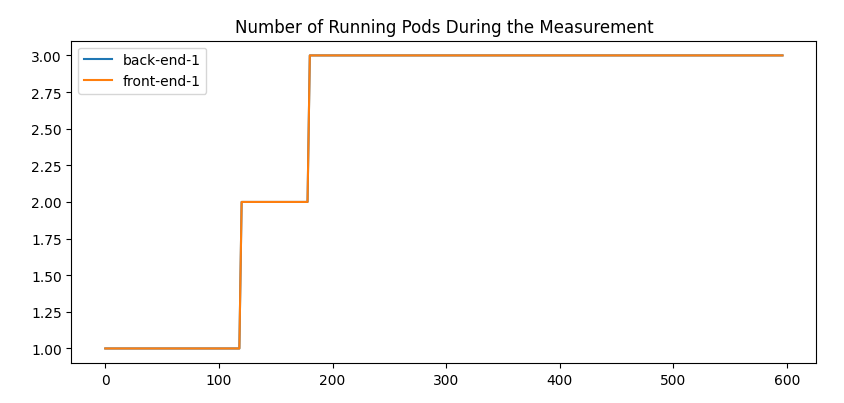
\includegraphics[width=150mm, keepaspectratio]{figures/HPA-scaling-in-the-same-time.png}
	\caption{HPA skálázóval történő mérés - 70\% cél CPU használat mellett}
	\label{fig:HPA-scaling-same-time}
\end{figure}

A bemutatott eredményekből adódik a kérdés, hogy mennyire általános jelenségről van szó, vagy csak a skálázó számára átadott paraméterek módosításával lehet-e javulást elérni.
Felmerült gondolatként, hogy a rendszer kezdeti állapotának változtatásával kaphatunk-e eltérő végeredményt.
Ezekre a kérdésekre kellett válaszokat keresni, hogy megállapításokat tegyünk a skálázó működését illetően.


\subsection{Mérés megismétlése, más indulási állapottal}
%----------------------------------------------------------------------------
További kérdés, hogy \aref{subsec:first-HPA-measure} fejezetben bemutatott rendszer skálázása mennyire változik a kiindulási állapottól.
Lehetséges, hogy az automatikus mechanizmus indulása előtti állapotnak kihatása lehet a skálázási döntésekre és emiatt eltérő helyzetekből indítva a végeredmények is eltérőek lesznek.

A kérdés megválaszolásához több különböző helyzetből elindítva is elvégeztem a méréseket. 
Minden indításnál más replikaszámot adtam meg az egyes alkalmazáskomponensek részére és ilyen állapotban kezdte el a skálázó a monitorozásukat.

Első esetben három frontend és egy darab backend indult, \aref{tab:1FE_1BE_chain_with_HPA} táblázatban bemutatásra kerülő paraméterek mellett.
A replikaszámok módosulását \aref{fig:HPA-scaling-from-3FE-1BE} gafikon tartalmazza.
Könnyen leolvasható, hogy a sárgával jelzett frontend podok mennyisége változatlan maradt a teljes mérés során, a skálázó döntései alapján nem volt indokolt a beavatkozás.
Ezzel szemben a kék színű backend folyamatosan került felskálázásra, egészen addig, amíg ki nem egyenlítődött a két típusú egység replikaszáma.
Ezzel együtt megkaptuk az eredeti mérés kimenetét, ahol szintén három, három egység került elindításra.
Annyi különbség észrevehető, hogy ez a folyamat valamivel gyorsabban végig tudott menni és a szimuláció kezdetét követő második percben már a végleges replikák futottak.

\begin{figure}[!ht]
	\centering
	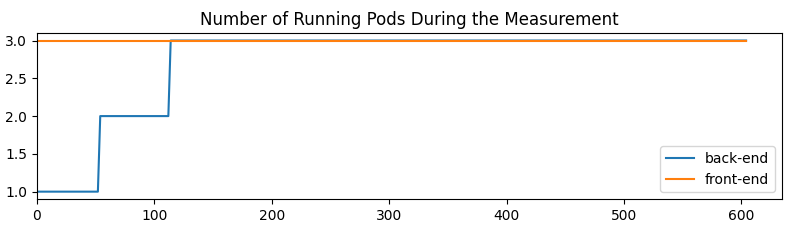
\includegraphics[width=150mm, keepaspectratio]{figures/HPA-scaling-from-3FE-1BE.png}
	\caption{HPA skálázóval történő mérés - 3 frontend és 1 backend kezdetben}
	\label{fig:HPA-scaling-from-3FE-1BE}
\end{figure}

Következő mérés elindítására az optimálisnak vélt erőforrás használathoz közelebbi állapotból került sor.
\Aref{fig:HPA-scaling-from-1FE-3BE} ábrán látható, hogy kezdetben egy frontend és három backend egység alkotta a rendszert. 
Ezután egy lépésben mindkét komponens replikaszáma növelésre került azonos időben.
Ezáltal el is érték az aktuális klaszterben szereplő ideális eloszlást.

\begin{figure}[!ht]
	\centering
	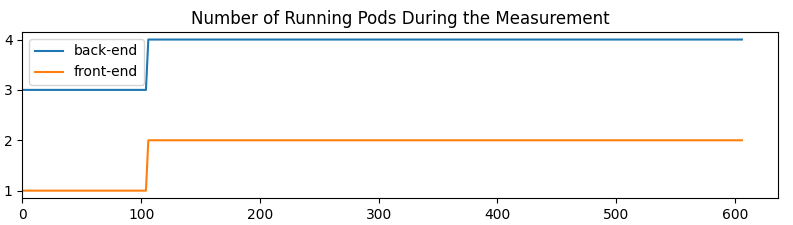
\includegraphics[width=150mm, keepaspectratio]{figures/HPA-scaling-from-1FE-3BE.png}
	\caption{HPA skálázóval történő mérés - 1 frontend és 3 backend kezdetben}
	\label{fig:HPA-scaling-from-1FE-3BE}
\end{figure}

Az elvégzett mérések és a bemutatott eredmények alapján kijelenthető, hogy a Kubernetes beépített skálázó által adott végeredmény nem független a klaszter eredeti állapotától.
A kapott erőforrás-allokációk az egyes alkalmazásegységek számára ideálisnak tartott állapottól való kezdeti távolságától nagymértékben függ.
Mivel minden skálázó, csak a saját hatáskörébe tartozó kapszulákat kezeli és azonos időben hoznak döntést, ezért az optimális állapotnak még a szabad erőforrások lefoglalása előtt be kell állni, mert utána erre már nem lesz képes.

% Ha optimális helyről indult: ott is maradt

\subsection{Processzorhasználati célérték konfigurálása}
%----------------------------------------------------------------------------
A korábbi mérek során felmerült, hogy azért történtek egyszerre a skálázások, mert a beállított cél processzorhasználati érték túl alacsonyan volt.
Az ideális érték meghatározása függ az alkalmazástól, illetve a beérkező kérések ingadozásától is.
Könnyen belátható, hogy minél nagyobb változásra számítunk, az időben annál nagyobb biztonsági tartalékot kell biztosítani az adott alkalmazásegységek részére.
Amikor fontos, hogy kiesés nélkül lehessen kiszolgálni az összes beérkező és várhatóan még beérkező igényt, akkor az eredeti mérésnél állított $70\%$-os érték jó kiindulást jelenthet.
Ezzel szemben a szimulációnk során a terhelés mértéke nem változott, a teljes mérés alatt azonos ütemben és azonos mennyiségű kérést intéztünk a hálózat felé.
Emiatt megfontolandó volt nem a kiindulási állapoton, hanem a célértéken is változtatni és megnövelni azt.
A megnövelt érték $90\%$ lett, mert így kellően nagy részét kihasználjuk a lefoglalt erőforrásnak és mégis marad egy $10\%$-os biztonsági tartalék.

A lefutott szimuláció végeredménye látható \aref{fig:HPA-scaling-in-the-same-time_90_percent} ábrán.
Leolvasható, hogy kezdetben egy kapszula futott a két alkalmazásból, és az első skálázásra együtt kerül sor.
Ezután viszont a fronted erőforrás használata nem lépte túl az előirányzott értéket és emiatt további növelésre nem volt szüksége.
Ezzel szemben a magas terheltségű backend képes volt fokozatosan skálázódni és a mérés végére négy darab replika futott belőle.
Ezzel a beállítással sikerült elérnie az elméleti optimumot a rendszerünknek.

\begin{figure}[!ht]
	\centering
	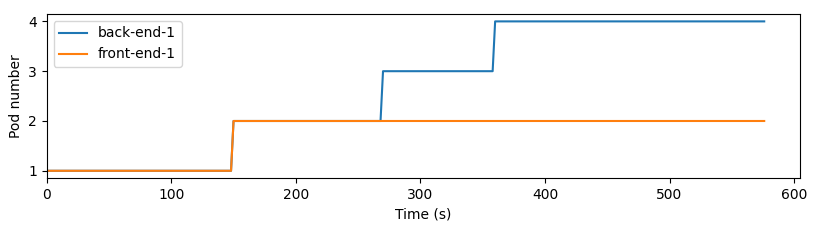
\includegraphics[width=150mm, keepaspectratio]{figures/HPA-scaling-in-the-same-time_90_percent_2.png}
	\caption{HPA skálázóval történő mérés - 90\%-os cél CPU érték}
	\label{fig:HPA-scaling-in-the-same-time_90_percent}
\end{figure}

Összefoglalva, a HPA konfigurációjával és a rendszer kiindulási állapotától függ az alapértelmezett skálázó által megtalált állapot.
Látható, hogy a rendelkezésre álló szűk erőforrások miatt fontos a körültekintő kezdeti konfiguráció, hiszen ezek hiányában csökken a kiszolgálások hatékonysága, feleslegesen használjuk és tartjuk lefoglalva a rendelkezésre álló erőforrásokat.

\subsection{Skálázás során jelentkező időkorlátok}
%----------------------------------------------------------------------------
%TODO 
A klaszter létrehozása közben a lehető legtöbb paraméter nem explicit módon konfigurálva, ezért az alapértelmezett paraméterek kerültek alkalmazásra.

Minél messzebb van az végső állapot annál tovább tarta annak elérése.